\documentclass[11pt]{report} % Dokumentenklasse

\usepackage[nomargin,inline]{fixme}
\usepackage[utf8]{inputenc} % Textkodierung: UTF-8
\usepackage[T1]{fontenc} % Zeichensatzkodierung

\usepackage[english]{babel} % Englische Lokalisierung
\usepackage{graphicx,float} % Grafiken
\usepackage[absolute]{textpos} % Positionierung

% Schriftart Helvetica:
\usepackage[scaled]{helvet}
\renewcommand{\familydefault}{\sfdefault}

\usepackage{calc} % Berechnungen
\usepackage{tabto} % Tabulatoren
\usepackage{parskip}
\usepackage{amsfonts}
\usepackage{amsmath,array,bm,mathtools}
\usepackage{xcolor}
\usepackage[backend=biber,sorting = none, style=numeric-comp, doi=false, isbn = false, url=false, giveninits=true]{biblatex}
\bibliography{Bibliography.bib}

\usepackage{pgfplots}
\pgfplotsset{compat=1.8,width = 5.5cm}
\usepgfplotslibrary{fillbetween}
\usepgfplotslibrary{groupplots}
\usepackage{pgfplotstable}
\usetikzlibrary{external}
%\tikzexternalize[prefix=./tikz/]


% Debugging:
%\usepackage{layout} % Layout-Informationen
%\usepackage{printlen} % Längenwerte ausgeben




\title{research internship report}
\date{\today}
\author{Seppich,Nicolas}

%%%%%%%%%%%%%%%%%%%%%%%%%%%%%%%%%%%%%%%%%%%%%%%%%%%%%%%%%%%%%%%%%%%%%%%%%%%%%%%%
% EINSTELLUNGEN
%%%%%%%%%%%%%%%%%%%%%%%%%%%%%%%%%%%%%%%%%%%%%%%%%%%%%%%%%%%%%%%%%%%%%%%%%%%%%%%%

% Seitenränder:
\newcommand{\SeitenrandOben}{43.5mm}
\newcommand{\SeitenrandRechts}{20mm}
\newcommand{\SeitenrandLinks}{20mm}
\newcommand{\SeitenrandUnten}{25.4mm}

\newcommand{\UniversitaetLogoBreite}{25mm}
\newcommand{\UniversitaetLogoHoehe}{1,31cm}

\usepackage[a4paper,
    top=\SeitenrandOben,
    bottom=\SeitenrandUnten,
    inner=\SeitenrandLinks,
    outer=\SeitenrandRechts,
    foot=0cm,
    head=0cm
]{geometry}

\textblockorigin{\SeitenrandLinks}{\SeitenrandOben} % Ursprung für Positionierung

\setlength{\parindent}{0pt}
%\setlength{\baselineskip}{32pt}
\setlength{\parskip}{\baselineskip}
\TabPositions{6cm}
\pagestyle{empty}


%%%%%%%%%%%%%%%%%%%%%%%%%%%%%%%%%%%%%%%%%%%%%%%%%%%%%%%%%%%%%%%%%%%%%%%%%%%%%%%%
% DOKUMENT
%%%%%%%%%%%%%%%%%%%%%%%%%%%%%%%%%%%%%%%%%%%%%%%%%%%%%%%%%%%%%%%%%%%%%%%%%%%%%%%%
\newcommand{\Titel}{Research internship report}
\newcommand{\Untertitel}{Measuring the acoustical impedance of liners using non equispaced prony like methods}
\newcommand{\BetreutVonPersonKTHS}{%
    Dr. Luck Peerlings}
\newcommand{\BetreutVonPersonKTHP}{%
    Prof. Dr. Tech. Hans Bodén}       
\newcommand{\BetreutVonPersonTUM}{%
    Prof. Dr. Wolfgang Polifke}
\newcommand{\BetreutVonLehrstuhlTUM}{%
    Professur für Thermofluiddynamik}
    \newcommand{\BetreutVonLehrstuhlKTH}{%
    Department of Aeronautical and Vehicle Engineering}
\newcommand{\EingereichtVon}{%
    Nicolas Seppich\\
    Matrikelnummer: 03671050\\
    Engineering Science at the Munich School of Engineering at TUM}
\newcommand{\EingereichtAmDatum}{%
    Datum}
\newcommand{\Ort}{%
    Place}
\newcommand{\Datum}{%
    Date}

%%%%%%%%%%%%%%%%%%%%%%%%%%
%Commands for matrices
%%%%%%%%%%%%%%%%%%%%%%%%%%

\newcommand*{\vertbar}{\rule[-1ex]{0.5pt}{2.5ex}}
\newcommand*{\horzbar}{\rule[.5ex]{2.5ex}{0.5pt}}

%%%%%%%%%%%%%%%%%%%%%%%%%%
%Starting the document
%%%%%%%%%%%%%%%%%%%%%%%%%%

\begin{document}
\begin{textblock*}{\UniversitaetLogoBreite}[1,0](\textwidth-1mm, 2cm-\SeitenrandOben)%
    \raggedleft
\includegraphics{./Deckblatt/Ressourcen/Universitaet_Logo_RGB.pdf}%
\end{textblock*}

\begin{center}
\begin{textblock*}{\textwidth}[0,0](0cm, 0cm)%
{\fontsize{18pt}{27pt}\selectfont\textbf{\Titel}}

\vspace*{12pt}
{\fontsize{24pt}{26pt}\selectfont\textbf{\Untertitel}}
\end{textblock*}
\end{center}


\vspace*{40mm}
\fontsize{15pt}{17.5pt}\selectfont%
\begin{center}
Research internship in the field of acoustics at the Markus Wallenberg Laboratory for Sound and Vibration Research at the KTH Stockholm.
\end{center}

\renewcommand{\baselinestretch}{1.47}
\normalsize\selectfont
\vspace*{17.1mm}

\textbf{Supervised at the KTH by:}\tab 
\begin{minipage}[t]{\textwidth-\CurrentLineWidth}
\BetreutVonPersonKTHP\\
\BetreutVonPersonKTHS\\
\BetreutVonLehrstuhlKTH\strut
\end{minipage}
\vspace*{-1mm}

\rule[-3.7mm]{\linewidth}{0.5pt}
\Ort{}, \Datum{}, Signature

\vspace*{6.3mm}
\textbf{Supervised at the TUM by:}\tab 
\begin{minipage}[t]{\textwidth-\CurrentLineWidth}
\BetreutVonPersonTUM\\
\BetreutVonLehrstuhlTUM\strut
\end{minipage} 
\vspace*{-1mm}

\rule[-3.7mm]{\linewidth}{0.5pt}
\Ort{}, \Datum{}, Signature

\vspace*{6.3mm}
\textbf{Submitted by}\tab 
\begin{minipage}[t]{\textwidth-\CurrentLineWidth}
\EingereichtVon
\end{minipage}
\vspace*{-1mm}

\rule[-3.7mm]{\linewidth}{0.5pt}
\Ort{}, \Datum{}, Signature


\chapter{Preface}
\section{Motivation}
Studying at university at undergraduate level usually means to a lot of students to study most of the time on a pure theoretical basis.
But since working in academia is supposed to combine both practical experimental and purely theoretical work, my department of the Technical University Munich provides the opportunity to gain insights into research topics during an optional research internship.
As part of my curriculum in engineering science at the Munich School of Engineering, I decided to complete this internship at the Marcus Wallenberg Laboratory for Sound and Vibration of the KTH in Stockholm, Sweden in the field of aero acoustics-
more specifically in the field of passive noise reduction using acoustic liners in aircraft engines. Here, I participated in a research project named the IMAGE project focussing on the optimization of these liners. 
During the 6 weeks of the internship, I could support the researchers and gain a lot of insights in specific tasks, which I am going to present in the following pages. 

\section{My field of activity} 
As the duration of the research internship was limited to period of 6 weeks, I participated in many tasks supporting the researchers instead of completing a single separate task.
These tasks are going to be explained in a detailed way in the following pages, but all in all encompassed the setup of experiments, research in literature, post processing the obtained data numerically with different methods and conducting uncertainty estimates.
I worked both practically in the laboratory and theoretically on fundamental theories of acoustics and maths.
As a member of a team of 3, I could also benefit from the expertise of my colleagues as well as acquiring helpful skills in team working. 

\subsection{Gathering of information concerning acoustics } 
The first days of the internship were used to acquire the demanded knowledge about acoustics, its governing equations and its methodologies.
In order to fulfil this purpose, the main task was to read several books such as 1, 2, 3 and gather several articles concerning the topic of acoustics, especially in flow acoustics. 
After a short period, I realized, that flow acoustics governs the combination of different subjects, which I already passed at TUM such as continuum mechanics, signal processing, control theory and thermodynamics.
With the acquired knowledge I was able to pass on to the main tasks. 

\subsection{Conduction of measurement series}
As I also participated in measurement series, several tasks needed to be fulfilled.
This included the preparation of the test set-up, preparation of the acoustical liners, calibration of the microphones and the conduction of test with or without flow.
Conducting these different steps in a specific order helped me to get a better understanding in how scientific tests are organized and which details need to be considered in order to get precise results. 

\subsection{Implementation of the equispacing algorithm}
\fxnote{Use the word implementation rather than development, the algortihm was already described in the paper. Also in the text, it could be good to explain equispaced in words such that it is clear what is meant.}
Basically my main task to be completed during the internship, was the implementation of an algorithm to postprocess the data obtained by the measurement in a special way. 
The purpose of the implemented algorithm is to approximate a function at equispaced positions. 
Equispaced positions means in specific a grid of uniform step size. 
The algorithm is necessary to meet the basic requirements for further postprocessing steps as determining the impedance numerically or using uncertainty estimate techniques to obtain reliable results.  
In order to fulfill this specific purpose, I conducted quite a lot of literature research to understand the governing background theory in the field of nonlinear approximation.
Several papers served as reference for the implementation of the algorithm. 
Due to the complexity this specific task consumed most of time during the internship.
In chapters 3 and 4 I will outline the algorithm and the obtained results in a more detailed way.
 
\chapter{Introduction} 
As acoustics is field of studies that bother our everyday lives, it is important to distinguish between wanted and unwanted acoustics.
While on one side acoustics are highly appreciated and essential in the field of communication, noise on the other side, is an unwanted side effect of many technical applications and can even lead to severe consequences for people.
Therefore, it is essential to develop efficient ways to reduce noise.

\section{Acoustic liners for passive sound reduction}
The research project, where I had the chance to get insights in during my internship, covered the topic of passive noise reduction methodologies with acoustic liners in aircraft engines.
In general, acoustic liners are technical components to damp sound waves using the principle of the so called Cremer's impedance. 
The Cremer's impedance is the optimal impedance, where locally reacting boundary conditions lead to a maximum attentuation of the lowest sound modes. \cite{Abom} 
More information about how to determine the Cremer's impedance will be provided in chapter 2.   

In aircraft engines the aeroacoustic liners are placed within the two critical areas of the engine - in the inlet and in the outlet, where most of the noise is generated. 	 
The principle set up of a liner consists of a porous or perforated top layer, a honeycomb structure and an impervious layer. 
Since the fundamental principle of passive noise reduction with sound absorbing materials in liners has been used for a long time, i.e. for more than 50 years, the focus is set on the optimization of several set ups and liner designs.


\section{The IMAGE project} 
In aero- engines, single-layer and double-layer liners with perforate and mesh facing sheets are standard elements to reduce noise, but for the optimization of novel liner designs and novel materials more research is required to understand their acoustic impedance characteristics.
This is where the project IMAGE comes into play.
The term IMAGE stands for Innovative Methodologies and technologies for reducing Aircraft noise Generation and Emission.
In detail, the project aims to investigate noise reduction technologies in aircrafts both in a numerical and experimental way in order to develop robust methodologies in this particular field of study.  
Whereas the main goal of the study conducted at the KTH at the Marcus Wallenberg Laboratory covers the characterization of the acoustical behaviour of porous materials in the reduction of fan noise in duct flow. 
The obtained results provide the basis references for further optimization steps of liners or for the further validation of numerical methods. 

\section{Characterisation of the impedance of liners in duct flows}
The experiments conducted at the MWL aim to determine the impedance spectra and consequently the acoustical behaviour of acoustic liners embedded in the walls of aero- engines.
Therefore, a model that simulates the acoustical behaviour of the liners in a duct flow is set up, where the applied sound spectrum is supposed to be of the same range as the one of the engines fan.  
The measured pressure provides the basis for post processing steps like the Prony method to examine parameters to deduce the impedance.
In order to understand further relations, the experimental setup and fundamental theories are shortly introduced in this section. 


\subsection{Experimental setup and measurements}
In our case, the experimental setup consists mainly of a rectangular duct with the liners embedded into the wall.
The following a will be graph be given outlining the schematic experimental setup. 

\begin{figure}[H]
\centering
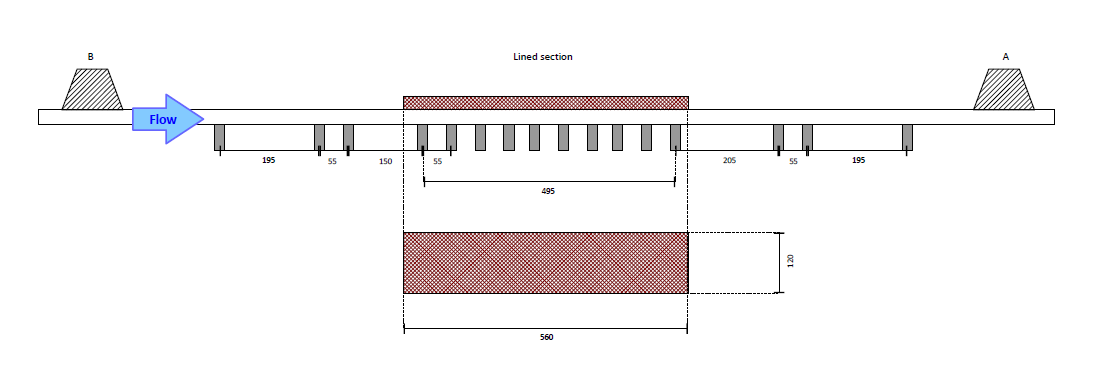
\includegraphics[scale=0.8]{./Figures/experimental_setup}
\caption{Schematic experimental setup}
\end{figure}

With the help of the illustrated 16 microphones and two loud speakers, that generates a sound field at specific frequencies, the impedance of the liners can be deduced using an inverse analytical method.
In this context, inverse analytical method means to deduce the acoustical impedance by measuring the sound field in a mean flow, in front of and after the lined section.
Therefore, 3 microphones and one speaker are placed respectively in front of and after the lined section, whereas the remaining 10 microphones face the liner.
The method is a non destructive method ensuring the liners further usage.
The governing relations between the measured pressures and how to determine the impedance is going to be given in more detail subsequently.


\subsection{The wave equation and its solutions}
\fxnote{Give references to the literature where you have taken the equations from}
Acoustic phenomena are based on wave propagation. As a consequence the governing equation is called the wave equation and is of the form: 

\begin{equation}
    \nabla^2p-\frac{1}{c^2}\frac{\partial^2p}{\partial^2t}  = 0 \label{eqn: waveeqn}
 \end{equation} 
 
with the pressure $p(x,y,z)$, the speed of sound $c$ and the time $t$

There are several ways to derive this partial differential equation including conservations laws like mass and momentum conservation, which are fundamental equations in thermodynamics and mechanics.
As the wave propagation is exposed to a duct flow in our case, further assumptions are necessary.
We will extend the wave equation \eqref{eqn: waveeqn} with a flow term, assuming a a mean flow U in only one direction- in our case the z-direction.
This allows us to make use of the relatively simple linearized modified wave equation: 

\begin{equation}
    \nabla ^2p-\frac{1}{c^2} \left( \frac{\partial}{\partial t}+U\frac{\partial}{\partial z} \right)^2p  = 0
\end{equation}   

Using complex notation the convective Helmholz wave equation is given by 

\begin{equation}
\nabla^2 p - \left(ik +M\frac{\partial}{\partial z}\right)^2p = 0
\end{equation},  

where $k=\frac{w}{c}$ denotes the wave number, $\omega$ the angular speed and $M=\frac{U}{c}$ the Mach number. 

The Helmholz equation has the general solution:
\begin{equation}
p(\textbf{x},t)=p^{-}e^{i(\omega t-k\textbf{x})}+p^{+}e^{i(\omega t+k\textbf{x})}
\end{equation}
with x the propagation vector. 

\subsection{Case of a rectangular duct}

\begin{figure}[H]
\centering
\includegraphics[scale=0.8]{./Figures/schematic_problem}
\caption{Schematic Problem using a rectangular duct}
\end{figure}

In our case of a rectangular duct and assuming a separable solution of the form  $p(x,y,z) = X(x)Y(y)Z(z)$, the convective Helmholz equation takes the form: 

\begin{subequations}
\begin{align}
0&=\frac{1}{X} \frac{d^2X}{dx^2}+\frac{1}{Y} \frac{d^2Y}{dy^2}+\frac{1}{Z} \frac{d^2Z}{dz^2} +k^2 -\frac{M^2}{Z}\frac{d^2Z}{dz^2}-\frac{2ik}{z} \frac{dZ}{dz}\\
0&=\frac{1}{X} \frac{d^2X}{dx^2}+\frac{1}{Y} \frac{d^2Y}{dy^2}+\frac{1}{Z} \frac{d^2Z}{dz^2}(1-M^2) -\frac{1}{Z}\frac{dZ}{dz}(2ikM)+k^2 	
\end{align}
\end{subequations}

where we used the rectangular coordinate system.
Both equations can be separated in terms of the respective direction taking into account, that each term only depends on one variable. 
The other terms can be considered as a constant. 
Therefore,  solving the remaining ordinary differential equations with the boundary conditions

\fxnote{Double check the second and third equation, they should involve the Y and X direction}
\begin{subequations}
\begin{align}
\frac{1}{z}\frac{d^2Z}{dz^2}(1-M^2)-\frac{1}{Z}\frac{dZ}{dz}(2ikM)+k^2-k_x^2-k_y^2&=0 \label{eqn: Zdirec} \\
\left( \frac{d}{dx^2}+k_x^2\right)X(x)&=0 \label{eqn: Ydirec} \\
\left( \frac{d}{dy^2}+k_y^2\right)Y(y)&=0 \label{eqn: Xdirec}
\end{align}
\end{subequations} 

lead to the determination of the wave numbers.   

\subsection{Boundary conditions to determine the wave numbers and the impedance}
In general, the acoustical impedance $z$ combines the two acoustical variables, the pressure $p$ and the velocity $u$ in the relation $z=\frac{p}{u}$. 
Whereas in our model including the mean flow $U$, the impedance is calculated using the the equations \ref{eqn: Zdirec} \ref{eqn: Ydirec} \ref{eqn: Xdirec} and boundary conditions. 

\begin{figure}[H]
\centering
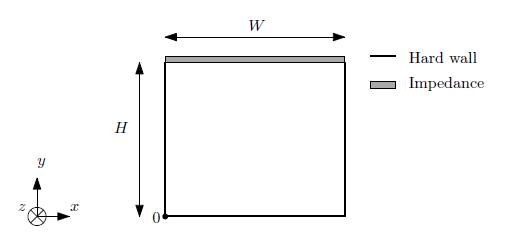
\includegraphics[scale=0.8]{./Figures/Boundary}
\caption{Exemplary crosssection of the duct}
\end{figure}

In axial direction the wavenumber is obtained by inserting the ansatz of the form: 

\begin{equation}
Z(z)\propto e^{-ik_z}
\end{equation}  

in the wave equation in z- direction \ref{eqn: Zdirec}.
This leads to following relation:

\begin{equation}\label{eqn: Impdet2}
    k_z = \frac{k}{1-M^2} \left( -M \pm \sqrt{1+(1-M^2)(k_x^2/k^2 + k_y^2/k^2)}\right)    
\end{equation}

For the wavenumbers in x or the y direction the boundary conditions need to be taken into account as seen in the schematic of the cross section.
In x direction, we assume both walls to be rigid resulting in:
 
\begin{equation}
\left.\frac{\delta}{\delta x}X\right\rvert_{x=0,x=W}=0
\end{equation}

In y direction the boundary conditions differ as seen in the schematic. 
Only on one side the boundary condition 
\begin{equation}
\left.\frac{\delta}{\delta y}Y\right\rvert_{y=0}=0
\end{equation}

holds.
On the other side an acoustic impedance $z_{ac}$ is given.
Solving the boundary conditions for the Ansatz for the solution in x and y direction of the form: 

\begin{subequations}
\begin{align}
X(x)&=A_xe^{ik_xx}+B_xe^{-ik_xx}\\
Y(y)&=A_ye^{ik_yy}+B_xe^{-ik_yy}
\end{align}
\end{subequations}
 
leads to following restriction on the wavenumber in x- direction: 
\begin{equation}
k_{x,m}=\frac{m\pi}{W}\\
\end{equation}

where the parameter n denotes the so called acoustical modes of the solution to to wave equation.\\
Solving the wave equation in y direction under the consideration of no reflections and the boundary conditions, the relation to determine the impedance is obtained: 

\begin{equation}\label{eqn: Impdet1}
    k_y \tan 2k_y H = \frac{i \rho_0 c_0^2}{\omega z_{ac}} \left[k-M_zk_z\right]^2
\end{equation}
Using the experimental data $k_z$ is measured. 
Then, from the first relation \ref{eqn: Impdet2} $k_y$ can be obtained under the consideration that the frequency is low enough that there are no modes in the $x$ direction $k_x = 0$, then with the second equation \ref{eqn: Impdet1} the acoustic impedance $z_ac$ can be obtained.

\section{Introduction to the Prony method}
In this section, the already mentioned Prony method is shortly introduced, which aims to recover the signal parameters $k_z$ from noisy sampled data to determine the experimental impedance of the liners as presented in the previous section.
As shown before, the acoustical field in z direction is assumed to be of the exponential form:
\begin{equation}
Z(z)\propto e^{-ik_z^j}
\end{equation}
where j denotes the mode shapes in z-direction.
Therefore, the Prony method also takes a similar model into account, which is of the form: 

\begin{equation}\label{eqn: expsum}
 p(x)=\sum\limits_{j=1}^M c_{j}e^{ik_z^jz} 
\end{equation}

where M denotes the number of acoustical modes in z direction. 

Summarizing, the prony method aims to recover analytically the pairwise different wavenumbers $k_z^{j}$ and complex coefficients $c_{j}$ of the acoustical modes present in the duct, given the function of complex pressures $p(z)$ at the microphone positions $z$.
In order to calculate the algebraic solution with least effort, it is necessary, that first the spacing of the sampled pressure $p(z)$ fulfils the Shannon-Nyquist theorem $\frac{4\pi}{spacing}>k_z$ and second that the data points are provided at an equispaced grid.
When the factors $c_j$ and $k_z^j$ are known, they can be related to the acoustic impedance with the previous equations (\ref{eqn: Impdet1})(\ref{eqn: Impdet2})
 
Beside the prony methods exist various other prony like methods to recover the signal paramters like the Esprit method (Estimation of Signal Prarametersvcia rotational Invariance Techniques) or the matrix pencil method described by \cite{Potts}.

\section{Problem: Facing uncertainties}
As measured data is always accompanied by uncertainties, it is also of importance to fit the uncertainty analysis into the basic modelling process.
Normally, this is a problem of non-trivial kind based on the right assumptions.
With the initial situation of only a few measurement points with quasi equispaced distances it is not possible to calculate uncertainties, where derivatives in the following form are demanded:

\begin{equation}
u_{i}(q)= \left\vert \frac{\partial q}{\partial x_{i}} \right\vert u( x_{i})
\end{equation}

where $u_{i}(q)$ denotes the uncertainty in the desired quantity $q$ due to the uncertainty in $x_{i}$.
Using the fact, that the microphone positions are not perfectly equispaced, allows us to approximate the wanted function at equipaced steps.
Thus, new data points are generated, which are not only necessary to calculate derivatives, but also to use the Prony method, where an equispaced grid is a basic requirement.
For these reasons an algorithm to approximate the function of complex pressure at an equispaced grid needed to be implemented. 
  
\chapter{Theory on the equispacing algorithm} 
As already seen, the approximation of the complex pressure function at an equispaced grid poses a basic requirement for the prony method as well as for using uncertainty estimates on the experimental data.
This is why, this chapter in particular focuses on the implementation and theories behind the equispacing algorithm, beginning with the basic ideas first followed by a detailed review. 

\section{Basic ideas}
The algorithm is based on the theory of \textit{non linear approximation by sums of exponentials and translates}, by \cite{Peter2011}.\\
So basically the idea behind the algorithm includes as before in the Prony method \eqref{eqn: expsum} to first approximate the function of obtained complex pressures in with a linear combination of complex exponentials.
In this case we use a non equispaced step size, giving us two types of coefficients to be determined - first the exponentials and second the complex coefficients $c_j$. 
With the help of so called window functions the complex coefficients are approximated using Fourier techniques, so that only the complex coefficients are unknown. 
This transforms the problem for each data point into a linear system of equations.
Solving this system in combination with using an equispaced grid lead to the approximation of the complex pressure at equispaced positions.
In the following sections the algorithm with its specific steps will be explained more in detail. 

\section{Generalization of the approximation with exponential sums}
As mentioned in the basic ideas, in a first step we generalize the sum of exponentials to a non equispaced grid $x_k \in{-\frac{1}{2},\frac{1}{2}}$:

\begin{equation} \label{eqn: nonequi exp}
 p(x_k)=\sum\limits_{j=1}^M c_{j}e^{ik^{j}x}
\end{equation}

with complex coefficients $c_{j} \neq 0$.
Basically, the goal of the algorithm is to determine the important coefficients fitting the linear combination of exponentials.
Therefore, further assumptions about the coefficients and the exponentials are needed.  

\section{Approximation of the coefficients $\bm{c_j}$ and determination of the coefficients $\bm{p_l}$}
In a second step of the algorithm, the complex coefficients $c_j$ are approximated by the Fourier transform of a so called window function from space to the wavenumber domain: 

\begin{equation}
c_{k} (\varphi) \coloneqq \int_{-\frac{1}{2}}^{\frac{1}{2}} \varphi (x) e^{-2 \pi kx} dx         
k \in \mathbb{N}
\end{equation}

\subsection{Window function}
In the section before, we introduced the term window function.
In general, a function is called a window function, which is zero valued outside a specific chosen interval.
So, as one can assume, there are quite a lot of possibilities to set up these window functions.
For our case the 1- periodization of a gaussian bell, as proclaimed in the paper of \cite{Peter2011} seemed to provide good results to work on with.
It is of the form: 
For a fixed $b \in \mathbb{R}^+$ and $L \in{\mathbb{N}}$ let:
\begin{equation}
\varphi(x)= \frac{1}{\sqrt{\pi b}} \sum\nolimits_{r \in \mathbb{N}}  e^{(L(x+r))^2/b}
\end{equation}
The truncated version of the gaussian bell takes the form: 
\begin{equation}
\psi(x)= \frac{1}{\sqrt{\pi b}} \sum\nolimits_{r \in \mathbb{N}}  e^{(L(x+r))^2/b}\chi_{(-m,m)}(L(x+r))
\end{equation}
with $1<m < \frac{L}{2}$ and
\begin{equation}
    \chi_{(-m,m)}(x)=
    \begin{cases}
      0, & \text{if}\ x\in (-m,m) \\
      1, & \text{otherwise}
    \end{cases}\notag
\end{equation} 
The question arose, why do we need to truncate the Gaussian bell? 
In the end, the truncation is used for further mathematical proofs to ensures that the window function is well localised in space, since it is zero valued outside a specific interval.
In general, the term well localised means, that a function is mainly concentrated within an interval and sufficiently small outside this interval.

\subsection{Determination of the coefficients $\bm{p_l}$}
To represent the governing exponentials, we will use the coefficients $p_l$ with $l \in{1,..,M}$    
This transforms in combination with the window function the equation \eqref{eqn: nonequi exp} to: 

\begin{equation}
p(x_{k})=\sum\limits_{l=1}^M p_{l}\psi(x_{k}-\frac{l}{L})\label{eqn: linear system}
\end{equation}.

Here, we aim to determine the coefficients $p_l$, since the coefficients $p_l$ are the last unknown coefficients and represent the unknown exponentials describing the the function of complex pressures.
So, in a third step, the parameters $p_l$ are going to be recovered solving the linear equation for all nodes of the following form: 
\begin{equation}
\bm{p(x)} = \bm{\Psi (x)} \bm{p}
\end{equation}

with the  vector $\bm{p(x)} \in \mathbb{C}^{K \times 1}$ providing information about the measured pressures at the non equispaced grid, the matrix $,\bm{\Psi (x)} \in \mathbb{C}^{K \times M}$ containing the window functions for the nodes  and the target vector of coefficients $\bm{p} \in \mathbb{C}^{M \times 1}$.
Specifically, this can be expressed as: 

\[
\begin{bmatrix}
	p(x_1) \\
	p(x_2) \\
	\vdots\\
	p(x_K)
\end{bmatrix} = 
\begin{bmatrix}
    \psi(x_{1}-\frac{1}{L})& \psi(x_{1}-\frac{2}{L})& \dots & \psi(x_{1}-\frac{M}{M}) \\
    \psi(x_{2}-\frac{1}{L})& \psi(x_{2}-\frac{2}{L})& \dots & \psi(x_{2}-\frac{M}{M}) \\
    \vdots &  &\ddots & \vdots \\
    \psi(x_{K}-\frac{1}{L})& \psi(x_{K}-\frac{2}{L})& \dots & \psi(x_{K}-\frac{M}{M}) \\   
\end{bmatrix}
\begin{bmatrix}
    p_1 \\
    p_2 \\
    \vdots \\
    p_{M}
\end{bmatrix}
\],

which can be solved easily using MatLab tools.

\section{Approximation at the non equispaced grid}
In the last step, the function of complex pressures is approximated at equispaced nodes. The grid can be equispaced, using a simple algorithm, which examines the average step size and generates a new grid with this information.
With the obtained coefficients $p_l$, the approximation will be completed adapting equispaced nodes into the equation \eqref{eqn: linear system}. 

\begin{equation}
 p(x'_{k})=\sum\limits_{j=1}^L h_{l}\varphi(x'_{k}-\frac{l}{L})=
\end{equation}. 

Again, this can be expressed as a matrix vector multiplication: 

\[
\begin{bmatrix}
	p(x'_1) \\
	p(x'_2) \\
	\vdots\\
	p(x'_K)
\end{bmatrix} = 
\begin{bmatrix}
    \psi(x'_{1}-\frac{1}{L})& \psi(x'_{1}-\frac{2}{L})& \dots & \psi(x'_{1}-\frac{M}{M}) \\
    \psi(x'_{2}-\frac{1}{L})& \psi(x'_{2}-\frac{2}{L})& \dots & \psi(x'_{2}-\frac{M}{M}) \\
    \vdots &  &\ddots & \vdots \\
    \psi(x'_{K}-\frac{1}{L})& \psi(x'_{K}-\frac{2}{L})& \dots & \psi(x'_{K}-\frac{M}{M}) \\   
\end{bmatrix}
\begin{bmatrix}
    p_1 \\
    p_2 \\
    \vdots \\
    p_{M}
\end{bmatrix}
\],

where $\bm{p(x')}$ denotes the approximated function of complex pressures at the equispaced nodes. 

\section{Variation of the algorithm using a single Gaussian bell}
The major goal of the algorithm is to approximate the function of complex pressures as good as possible.
Since the truncation of the Gaussian was used to be well localised in frequency and space to proof convergence, we were interested to test the non truncated version of the Gaussian Bell.
So, we slightly changed our starting function \eqref{eqn:truncatew} and simply used this form of the original Gaussian window function of a non 1- periodical form:
  
\begin{equation}
 p(x)=\sum\limits_{j=1}^L h_{l}\varphi(x-\frac{l}{L})
\end{equation}

with $\varphi$ is the original Gaussian bell function: 

\begin{equation}
\varphi(x)= \frac{1}{\sqrt{\pi b}}  e^{x^2/b}
\end{equation}

where l denotes the shift parameter.
In essence, the rest of the main algorithm remained basically the same.
It is still the goal to deduce the coefficients $h_{l}$ by solving the linear system of equations: 
\begin{equation}
p(x_{k})=\sum\limits_{j=1}^L p_{l}\varphi(x_{k}-\frac{l}{L})
\end{equation}
and then approximate the function with remained coefficients at the equispaced grid: 
\begin{equation}
p(x'_{k})= \sum\limits_{j=1}^L h_{l}\varphi(x'_{k}-\frac{l}{L}) \notag
\end{equation}


\chapter{Results and conclusion}
In this chapter, the results concerning the usage of the equispacing algorithm are going to be outlined in detail. 
The first section is devoted to the reconstruction of the function of complex pressure.
Here, we aim to compare the two before mentioned variations of the equispacing algorithm, with or without the truncated window function. 
Whereas the second section deals with the results of applying the algorithm to experimental data using uncertainty estimates. 
 
\section{Numerical experiments}
Since two different variations of the equispacing algorithm exist, it was a necessary step to analyse the numerical behaviour of both variants.
A test class with possible numbers of scenerios equations was implemented, where the  
algorithm could be verified under realistic acoustical waves and under a nonequispaced grid.
In essence, the test makes use of a simple known steady wave equation of the form

\begin{equation}
p(x)= \sum e^{kx},
\end{equation}

where the test data is obtained inserting a non equispaced grid. 
The equispaced grid is randomly generated but is kept in a specific range such as 10 percent of the step size. 
Applying now the algorithm to this test data and comparing the obtained results with the known function values delivers the approximation error in the complex domain.

\subsection{Results of using the truncated window function}
In the following plot the results using the truncated window function can be examined. 

\begin{figure}[H]
\centering
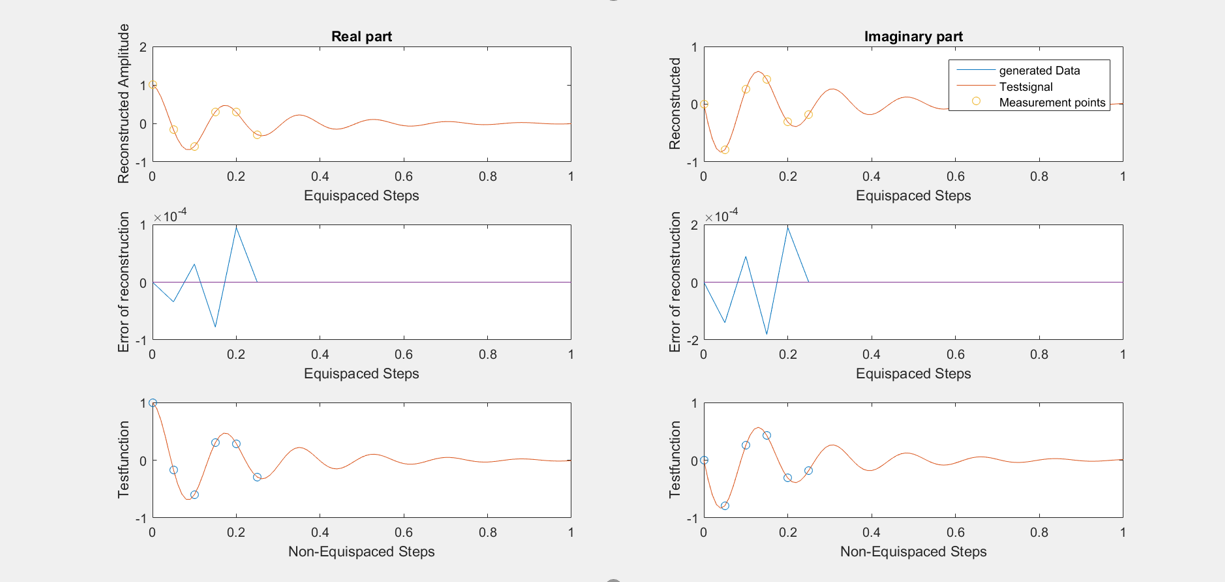
\includegraphics[scale=0.8]{./Figures/plot_trunc}
\caption{Results of using the truncated window function with the parameters $b=12.3$ and $m=3$ as proclaimed in }
\end{figure}

This example shows in the first row the reconstructed function of complex pressures approximated at equispaced steps, separated in real and complex part. 
Here, it is quite difficult to distinguish between the the test function and the the approximated function. 
Therefore, a plot is shown in the second row displaying the error between the test function and the approximated function. 
According to plot the error is smaller than $10^{-2}$, which provides quite a robust result for an non equispaced grid of 5 percent deviations, which is displayed in the last row.


\subsection{Results of using a single Gaussian bell}
In comparison to the first plot, the second plot provides information about the numerical properties of using a single Gaussian bell using the same equispaced grid as before.

\begin{figure}[H]
\centering
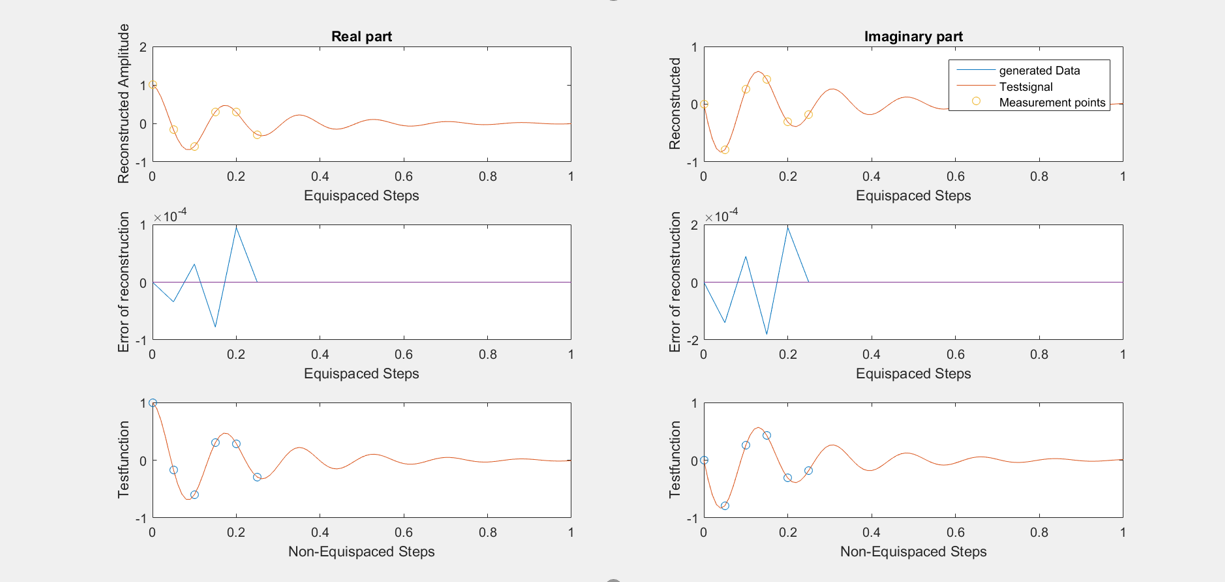
\includegraphics[scale=0.8]{./Figures/plot_trunc}
\caption{results of using the gaussian bell with the parameters $b=12.3$}
\end{figure}

This plot shows as the first example the reconstructed function of complex pressures approximated at equispaced steps, separated in real and complex part.
As before, the numerical errors are quite small.
In this case ten times smaller than before. 
So, the single Gaussian bell provides even better results than the truncated version. 


\section{Results of using uncertainty estimates on experimental data}
As mentioned before, the implemented algorithm is supposed to fulfil two purposes. 
Beside the reconstruction of the pressure function at equispaced positions, the generated data provides the base for uncertainty estimates on the calculated impedance of the acoustical liners. 
Therefore, the equispacing algorithm could be included in the work of my colleague Luck Peerlings on uncertainty estimates \cite{Luck}. 
This led to the following results: 

\begin{figure}[H]
\centering
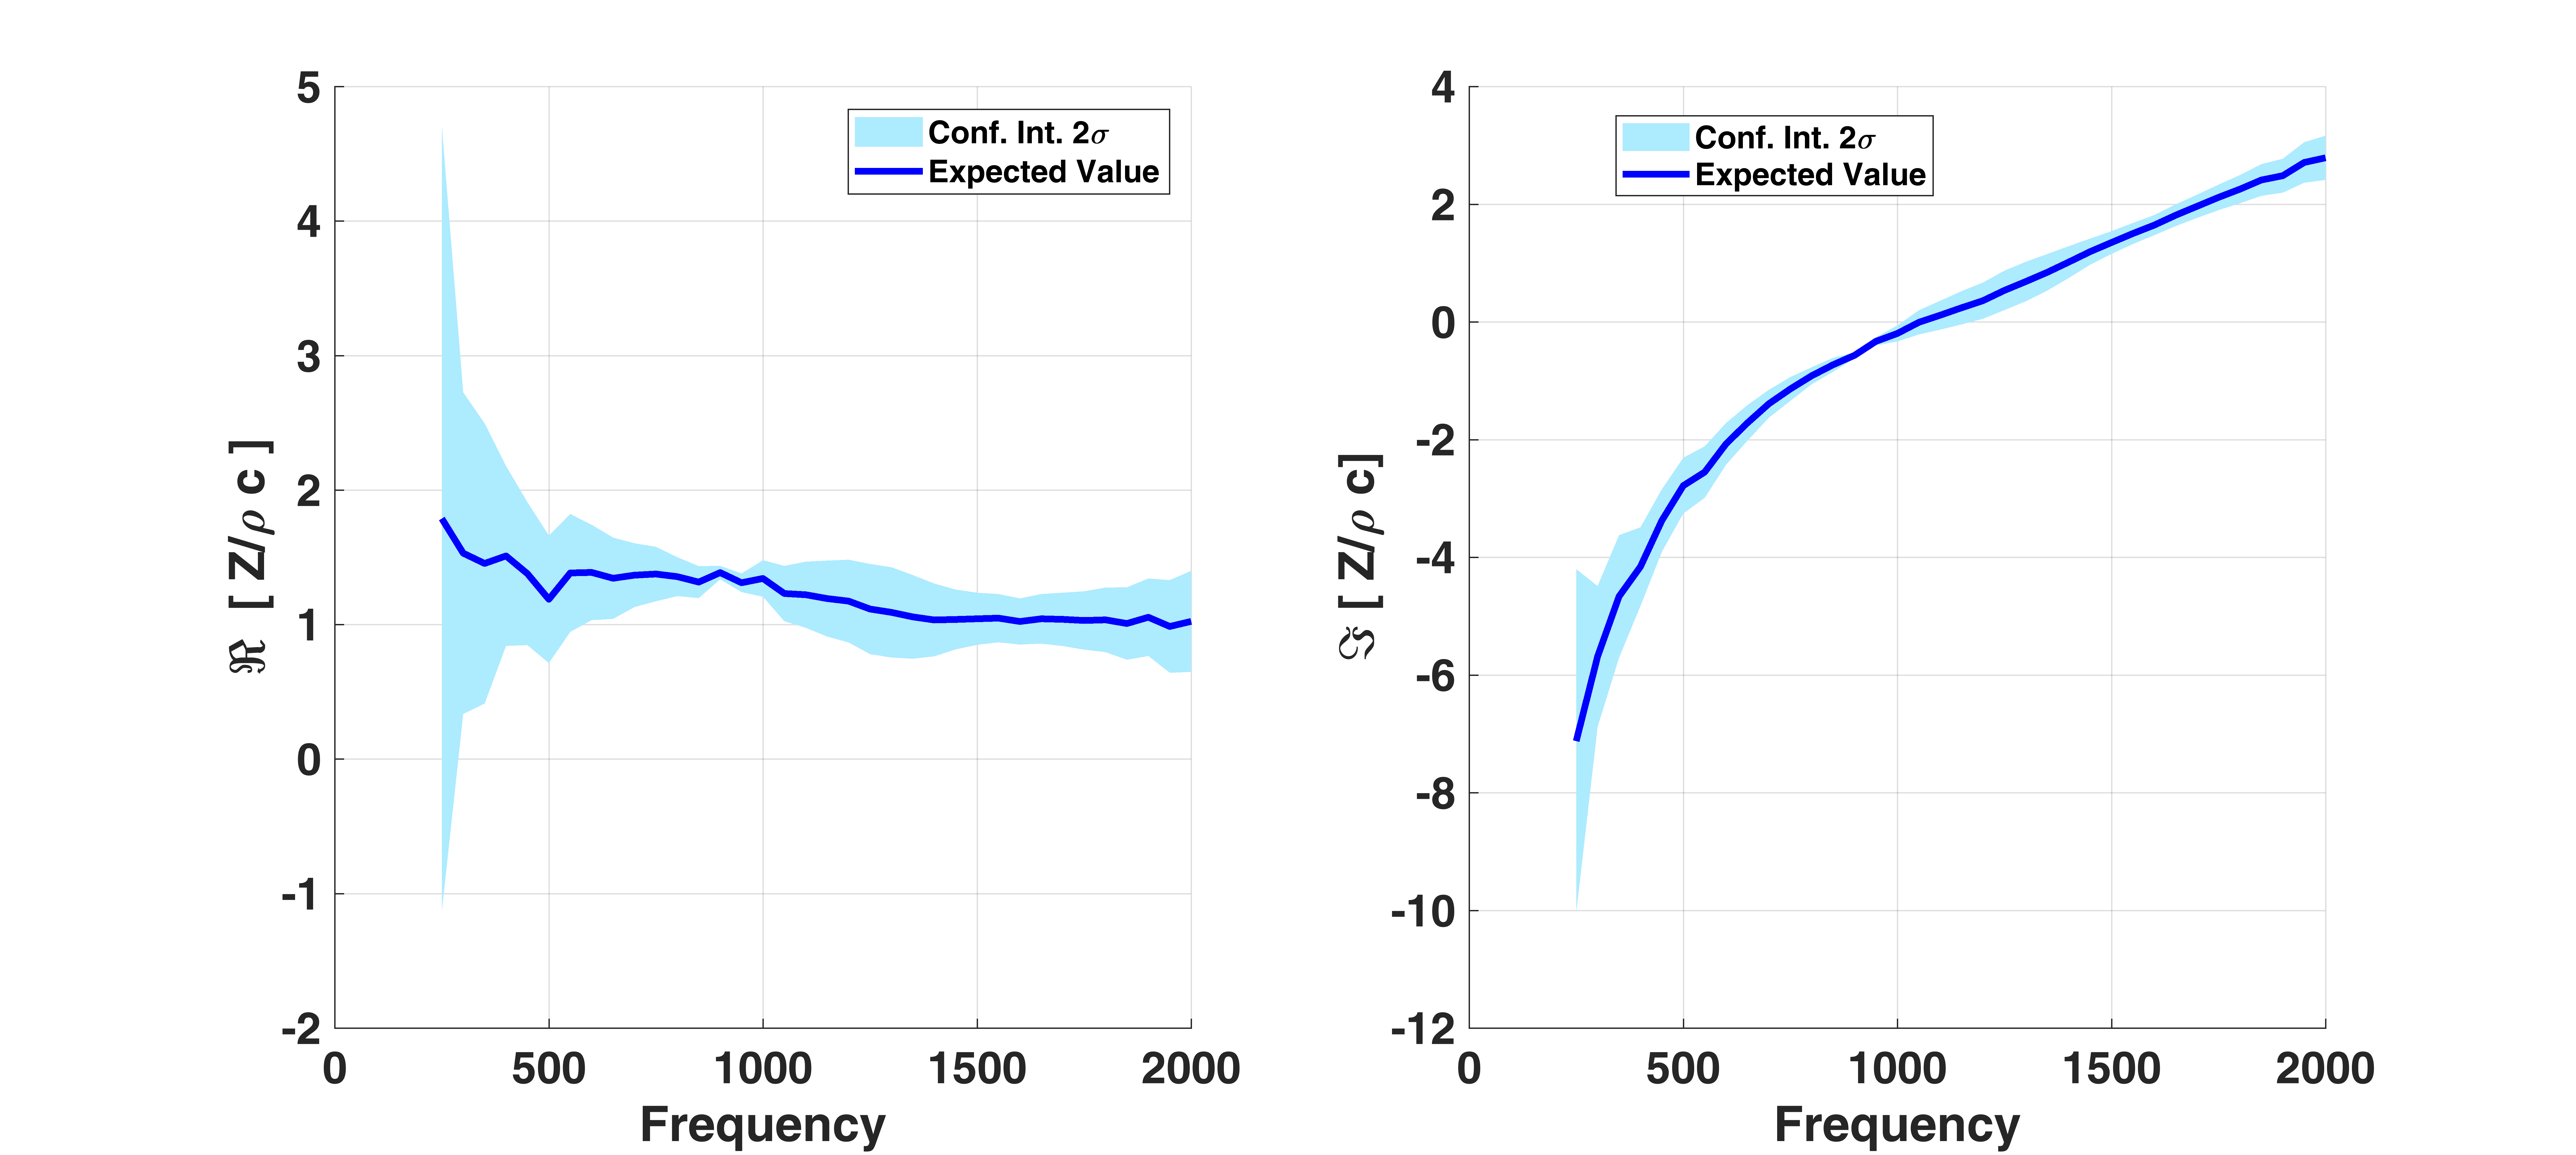
\includegraphics[width=1\textwidth]{./Figures/UncertaintyFigure}
\caption{Example of an uncertainty calculation of the impedance of a liner with flow.}
\end{figure}

This graph illustrates the determination of the acoustical impedance using uncertainty estimates with a specific level of confidence.
The real part is shown on the left side, whereas the imaginary part is shown on the right side. 

 
\section{Conclusion}
On the scientific point of view, on may conclude, that the equispacing algorithm fulfils successfully the stated requirements and goals.
It has been shown that it provides quite a robust solution to the approximation problem of a function given on a non equispaced grid. 
Also, it has been shown that the algorithm is adaptable to often used uncertainty estimates on experimental data and thus provides additional information on the data.  
Therefore, the equispacing algorithm can be successfully used in the framework of analysing the experimental data to determine the acoustical impedance. 

On a personal point of view, the research internship has been a great experience to me.
Beside discovering the interesting subject of acoustics, I could also benefit from the productive atmosphere given at the university and from the expertise of my colleagues. 
I really enjoyed being part of great team and the interesting IMAGE project. 
  
%\begin{figure}[b]% Reflection coefficient   
%    \centering
%    \begin{tikzpicture}[scale = 1]
%        \begin{axis}[
%                xlabel={Frequency [kHz]},
%                ylabel={$|\hat{\mathcal{R}}|$ [-]},
%                axis on top,
%                xmin = 0, xmax = 4,
%                ymin = 0.96, ymax = 1,
%                minor tick num = 5,
%                grid
%            ]
%            \addplot[
%                    color =  red,
%                    line width = 0.5,
%                ] 
%                table[x expr= \thisrow{f}/1000, y={mag} ] {./Data/UncertaintyAnalysis.txt};
%            \addplot[line width = 1] table[x expr= \thisrow{f}/1000, y={create col/linear regression={y=mag}}] {./Data/UncertaintyAnalysis.txt};
%        \end{axis}
%    \end{tikzpicture}
%    \begin{tikzpicture}[scale = 1]
%        \begin{axis}[
%                xlabel={Frequency [kHz]},
%                ylabel={$\angle \hat{\mathcal{R}}$ [deg]},
%                axis on top,
%                xmin = 0, xmax = 4,
%                ymin = -5, ymax = 5,
%                minor tick num = 5,
%                grid
%            ]
%            \addplot[
%                    color =  black!90,
%                    line width = 0.5,
%                ] 
%                table[x expr= \thisrow{f}/1000, y={phase} ] {./Data/UncertaintyAnalysis.txt};
%        \end{axis}
%    \end{tikzpicture}
%    \caption{Measured reflection coefficient of the rigid plate. In blue the measured value and red gives the 95\% confidence intervals}
%    \label{fig:ReflCoeff}
%\end{figure} 
%
%\begin{figure}
%\centering
%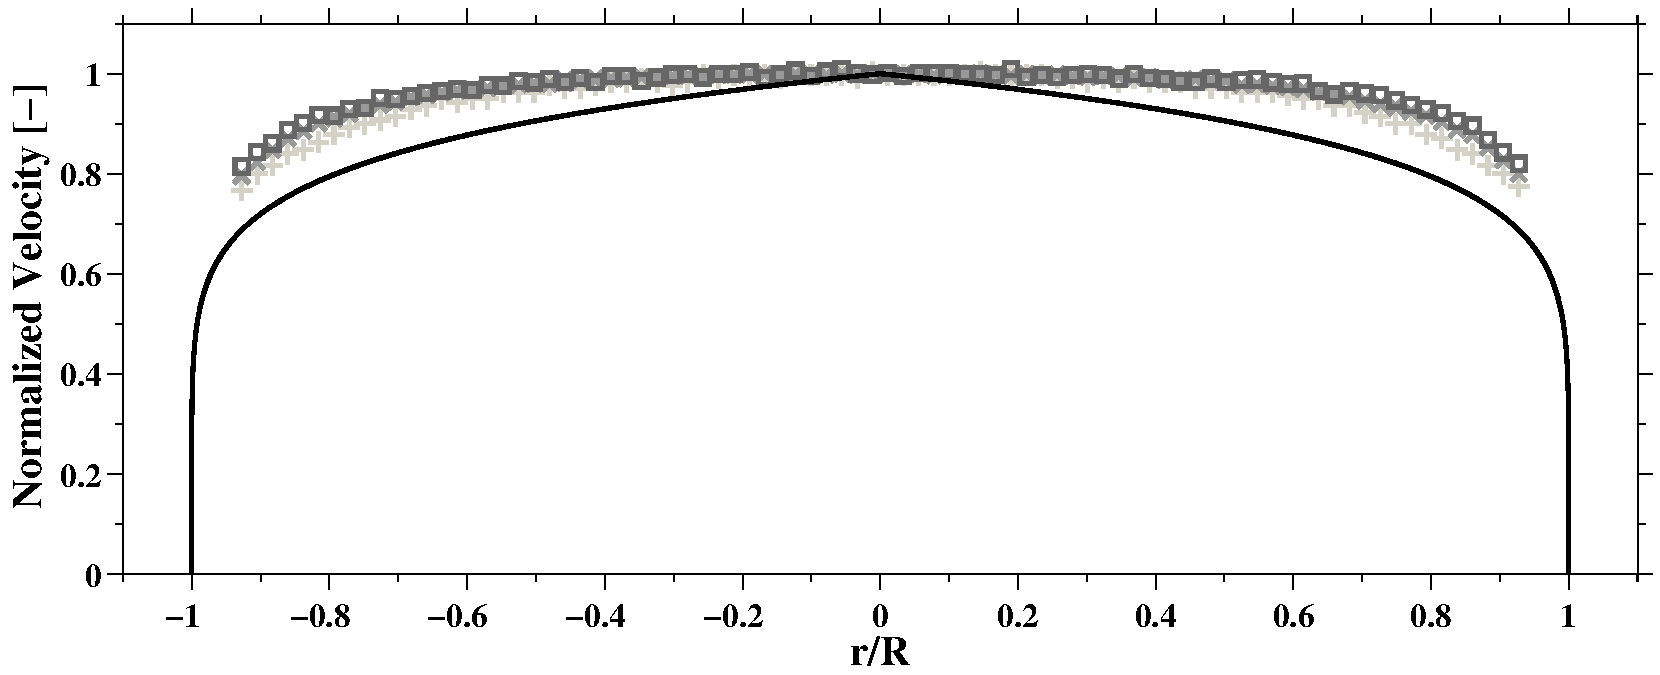
\includegraphics[width = 0.3\textwidth]{./Figures/FlowProfile_Large}
%\caption{Test 123}
%\end{figure}


\cite{Peter2011}
\cite{Mungur1969}
\printbibliography


\end{document}


